\section{Implementierung des SmBasicSafeRetries}

Der nächste DEA verwendet den SmBasic als Grundlage und soll das Problem des vorzeitigen Abbruchs verhindern. Dabei sollen keine neuen Inkonsistenzquellen eingeführt werden. 

\paragraph*{Netzwerkfehler}
Für alle Transaktionen, die nicht zu einer Änderung des Systemzustands eines Teilnehmerservices führen, können Retries im Falle eines Netzwerkfehlers eingeführt werden. Dazu gehören \textit{GetArticleData} und \textit{GetShipmentStatus}. 

\paragraph*{Lastfehler}
Behindern sich mehrere parallele lokale Transaktionen innerhalb eines Teilnehmerservices, kommt es zu einer Race Condition (Wettlaufsituation). Dabei gewinnt die erste lokale Transaktion T1 und kann wie gewohnt abgeschlossen werden. Alle lokalen Transaktionen, die innerhalb der Bearbeitungszeit von T1 auf die gesperrten Ressourcen zugreifen, schlagen fehl. Die aus diesem Fehler resultierende Response enthält den Http-Statuscode 429 und wird vom Koordinator auf ein entsprechendes Ergebnis gemappt. Dieses Verhalten ist für den StockService und die BankServices implementiert. 

Antwortet ein Service mit einer solchen Response, ist der Fehler durch einen Retry auflösbar. Das bedeutet, dass für die lokalen Transaktionen \textit{BlockArticles}, \textit{RemoveMoney}, \textit{AddMoney} und \textit{StartShipment} ein Retry eingeführt werden kann. Ebenso kann diese Stategie auf alle zugehörigen Kompensierungen angewendet werden.

\paragraph*{DEA SmBasicSafeRetries}
Aus den beschriebenen Anpassungen ergibt sich der SmBasicSafeRetries in \cref{fig:SmBasicSafeRetries}. 

\begin{figure}[h!]
	\centering
	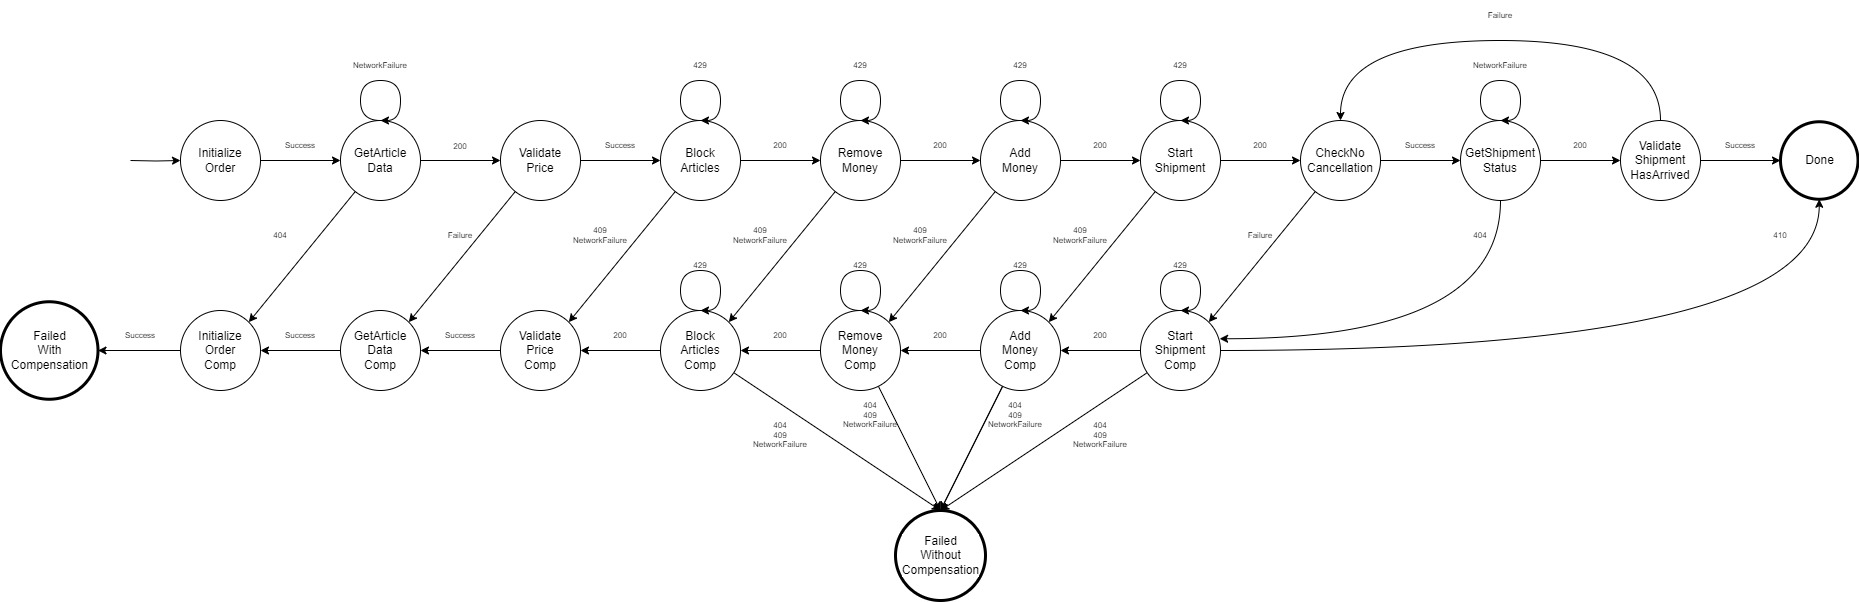
\includegraphics[width=\linewidth]{figures/ChapterVersuchsdurchführung/sm_basic_safe_retries.jpg}
	\caption{SmBasicSafeRetries}
	\label{fig:SmBasicSafeRetries}
\end{figure}
\FloatBarrier

\subsection{StateAnalysisResult}

\paragraph*{Testfall FinishOrders}
%TODO
\begin{center}
	\fontsize{9}{12}\selectfont
	\begin{longtable}[h]{|p{5cm}|p{1cm}|p{1cm}|p{1cm}|}
		\hline
		Messwert & S1 & S2 & S3 \\ \hline
		\endhead
		\caption{StateAnalysisResult SmBasicSafeRetries im Testfall FinishOrders}
		\label{tab:smbasicsaferetries_stateanalysisresult_finishorders}
		\endfoot
		successfull\-Percentage & 1.0 & 0.66 & 0.4 \\ \hline
		finished\-Percentage & 1.0 & 1.0 & 1.0 \\ \hline
		pending\-Percentage & 0.0 & 0.0 & 0.0 \\ \hline
		failedWithCompensation\-Percentage & 0 & 0.29 & 0.46 \\ \hline
		failedWithoutCompensation\-Percentage & 0.0 & 0.05 & 0.15 \\ \hline
		hasCorrectEndstate\-Percentage & 1.0 & 0.66 & 0.4 \\ \hline
		containsAllExpectedLogs\-Percentage & 1.0 & 0.66 & 0.4 \\ \hline
		isSuccessfullTestInstance\-Percentage & 1.0 & 0.66 & 0.4 \\ \hline
	\end{longtable}
\end{center}
\FloatBarrier

\paragraph*{Testfall CancelOrders}
%TODO
\begin{center}
	\fontsize{9}{12}\selectfont
	\begin{longtable}[h]{|p{5cm}|p{1cm}|p{1cm}|p{1cm}|}
		\hline
		Messwert & S1 & S2 & S3 \\ \hline
		\endhead
		\caption{StateAnalysisResult SmBasicSafeRetries im Testfall FinishOrders}
		\label{tab:smbasicsaferetries_stateanalysisresult_cancelorders}
		\endfoot
		successfull\-Percentage & 1.0 & 0.66 & 0.4 \\ \hline
		finished\-Percentage & 1.0 & 1.0 & 1.0 \\ \hline
		pending\-Percentage & 0.0 & 0.0 & 0.0 \\ \hline
		failedWithCompensation\-Percentage & 0 & 0.29 & 0.46 \\ \hline
		failedWithoutCompensation\-Percentage & 0.0 & 0.05 & 0.15 \\ \hline
		hasCorrectEndstate\-Percentage & 1.0 & 0.66 & 0.4 \\ \hline
		containsAllExpectedLogs\-Percentage & 1.0 & 0.66 & 0.4 \\ \hline
		isSuccessfullTestInstance\-Percentage & 1.0 & 0.66 & 0.4 \\ \hline
	\end{longtable}
\end{center}
\FloatBarrier